\begin{figure*}[t!]
~\hrule~
\begin{minipage}{.53\linewidth}
\small
 \begin{tabular}{p{0.95\linewidth}} 
 On the right-hand-side is a tree
 generated by iterative dichomization. 
 This tree can be read like a nested if-then-else statement; e.g.
 \begin{itemize}
     \item Lines 3 and 8 show two branches for lines of code (denoted here as {\em `\$loc}) below 698 and above 698.
     \item Any line with a colon ":" character shows  a  leaf  of  this  nesting.   For  example,  if  some  new  code module is passed down this tree and falls to the line marked in \textcolor{orange}{{\bf orange}},  the colon on that line indicates a prediction that this module has a 100\% chance of being defective. 
     \end{itemize}
Using this tree,
 XTREE looks for a nearby branch that has a lower chance of being defective. Finding the \textcolor{green}{{ green}} desired  branch,  XTREE reports a bad smell threshold for that module that is the delta between the \textcolor{orange}{{\bf orange}}  current branch  and   \textcolor{green}{{ green}} designed branch.
 In this case, that threshold relates to:
 \begin{itemize}
     \item Lines of code and comments ({\em lcom}) 
     \item The cohesion between classes ({\em cam}) which measures similarity of parameter lists to assess the relatedness amongst class   methods.
     \end{itemize}\\ 
 \end{tabular}
 \end{minipage}~~~~
 \begin{minipage}{.45\linewidth}
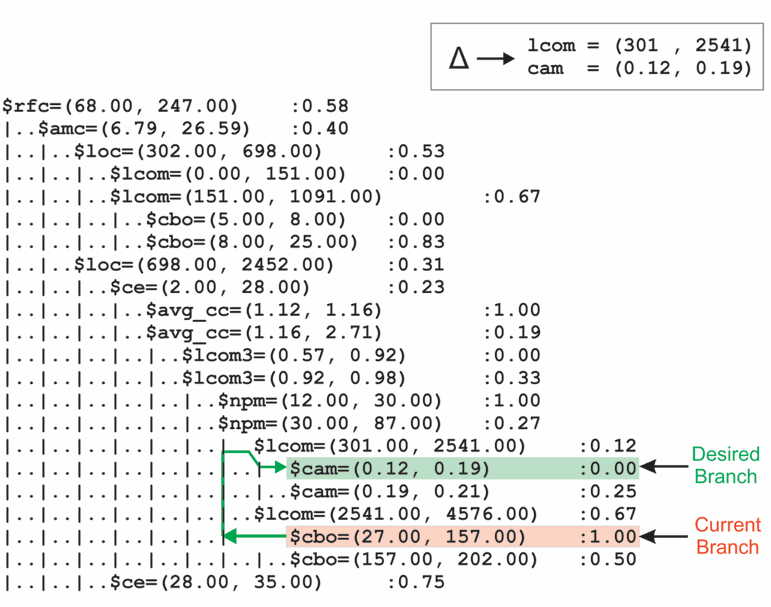
\includegraphics[width=\linewidth]{XTREE_samp.png}
\end{minipage}
~\hrule~
 \caption{A brief tutorial on XTREE.} \label{fig:xtree_samp}
\end{figure*}